

\section{Project Introduction \& Objectives}
\subsection{Introduction}

\begin{frame}[fragile,allowframebreaks]\frametitle{Motivation}
\begin{itemize}
\item The application that is going to be developed is web-oriented and focused on real time
communications. 
\item This kind of technology has been developed by Google in order to use on its browsers, thing that make easier
the fact no plugins and extensions are required to install in order to use it.
\item To start,  we will have to treat many aspects: % After researching we realize that we had to learn....
% En la lista solo se nombran, se tendrán que explicar en la presentación.
  \begin{enumerate}
  \item WebRTC API's and technologies.
  \item HTML language.
  \item JavaScript language.
  \item Callback concept.
  \item Server made with Node.js technology.
  \item Signaling process.
  \item Latex.
  \end{enumerate}
\end{itemize}
\framebreak
\begin{itemize}

\item Other related knowledges are needed, those that have been acquired during this years
at the university, thing that will make easier all the absorption of concepts above:

% En la lista solo se nombran, se tendrán que explicar en la presentación.
  \begin{enumerate}
  \item Object Oriented Programming.
  \item Multimedia coding.
  \item Audio/video concepts.
  \item Telematic concepts.
  \item Unix/Linux environment.
  \end{enumerate}

% Aqui se explicaria todo el proceso inicial de busqueda de informacion, como y donde la hemos buscado
\item The main goal of this project is help us to get started with WebRTC by researching and
understanding this technology and finally trying to develop a simple WebRTC site from scratch.

\end{itemize}
\end{frame}
\clearpage

\subsection{Objectives}
\begin{frame}[fragile]\frametitle{Objectives}
\begin{itemize}

\item Develop a web application through an expanding technology as WebRTC to:
  \begin{enumerate}
  \item Establish multimedia communication between peers.
  \item Room treatment.
  \item Text chat communication.
  \item File sharing.
  \end{enumerate}
  
\item The application should have the following objectives:%After all, our project will have the following 
%%objectives which have been defined taking into account
%the introduction themes to treat, so it was decided that the application had at least:

%Aqui se tendrian que explicar un poco que haria cada especificacion a crear. En la lista solo se nombran, pero se tendran que explicar.
  \begin{enumerate}
  \item A Node.js Server.
  \item Web-page made with html and JavaScript code.
  \item Handle streams.
  \item HTTPS secure connection. %Introducir/Explicar el porque del cambio de http a https.
  \item File Sharing.
  \end{enumerate}
\end{itemize}
\end{frame}

\section{WebRTC overview}
\subsection{A few of history...}
\begin{frame}[fragile]\frametitle{History}
\begin{itemize}

\item The web evolution...
  \begin{enumerate}
  \item 1990:Navigation by HREF-based hyperlinks.
  \item 2000: XMLHttpRequest (XHR), no need to update their content. Allow server-based web services like Facebook, Gmail, etc..
  \item Nowadays: NO servers required to transmit data between peers.
  \end{enumerate}
\end{itemize}
\end{frame}
\clearpage


\begin{frame}[fragile]\frametitle{Overview}
\begin{itemize}

\item Direct peer to peer communications should provide:
\begin{enumerate}
 \item Lower latency.
 \item Multiplayer gaming.
 \item Video/audio streaming.
 \item Sensor data feeds.
 \item Secure P2P connections. % Permiten itenrcambio info privada, sin necesidad de servidores, 
 
\end{enumerate}
\item So it allows the fact of exchanging information privately without being managed by intermediary servers. 
It introduces a way to create new types of services and applications.

\item This is just a brief overview of how WebRTC can be used.
\end{itemize}
\end{frame}
\clearpage

\subsection{Pros and cons}
\begin{frame}[fragile]\frametitle{Trade Off}
\begin{itemize}
\item Advantages:
  \begin{enumerate}
  \item No plugins required. %just update your browser.
  \item Only a handshaking process (Signaling). % between the server and the participants
  \item No server required to exchanging data.
  \item File sharing or text chat (Data channel).
  \item Better encryption.% The traffic is encrypted between peers, so it means that
  %if you are being attacked by a MiD (man in the middle) it’s really harder to
  %break it down.
  \end{enumerate}

\item Drawbacks:
  \begin{enumerate}
  \item Vulnerable on the signaling process.% One must be careful to not to use passwords or shared secrets at the signaling process because at this step data is not encrypted.
  \item Not supported for all browsers. %IE & Safari are not supported.
  \item Mobiles are not supported yet. %No native mobile support.
  \item Hard to scaling. %Large video calls are not well scaled. It means that if
  %you want to do a multi chat connection, each user has to have a peer to peer
  %connection with all the other users. Right figures are 4 to 8 users.
  \end{enumerate}
\end{itemize}
\end{frame}
\clearpage

\begin{frame}[fragile]\frametitle{Browser support}

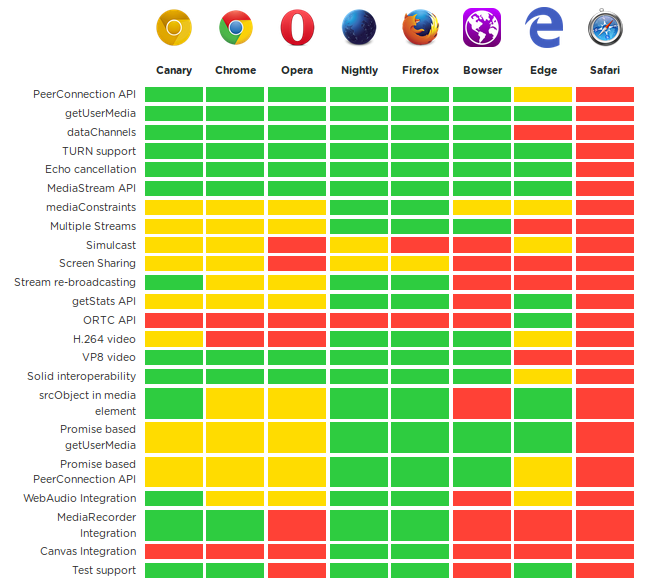
\includegraphics[width=0.8\textwidth]{\webrtcdir/figures/figuras_utilizadas/webrtc_browsers_state1.png}

\end{frame}

\section{Signaling}
\begin{frame}[fragile]\frametitle{Signaling Overview}
\begin{itemize}
 
\item Analogy:
\item Private Branch exchange
%%This is an analog process like the early days of telephone. When you wanted to call somebody, the signal is picked up by telephone operator, 
%%which used to patch the signal with the final user. It was like a \textbf{Manual Handshake} between two parties.

\item Signaling is an extremely important part of webRTC. In order for a WebRTC application to set up a 'call', its clients need to exchange information:
  \begin{enumerate}
  \item Session control messages used to open or close communication.
  \item Error messages.
  \item Media meta data such as codecs and codec settings, bandwidth and media types.
  \item Key data, used to establish secure connections.
  \item Network data, such as a host's IP address and port as seen by the outside world.
  \end{enumerate}
\end{itemize}
\end{frame}
\clearpage

\begin{frame}[fragile,allowframebreaks]\frametitle{Signaling}
 
\begin{columns}
\begin{column}{0.48\textwidth}

\begin{itemize}
\item Signaling methods and protocols are not defined on the WebRTC standards
in order to maximize compatibility with established technologies. 
\item The JavaScript Session Establishment Protocol (JSEP) defines an approach 
for the fully application but excludes the signaling methods to use.
\end{itemize}
\end {column}
\begin{column}{0.48\textwidth}
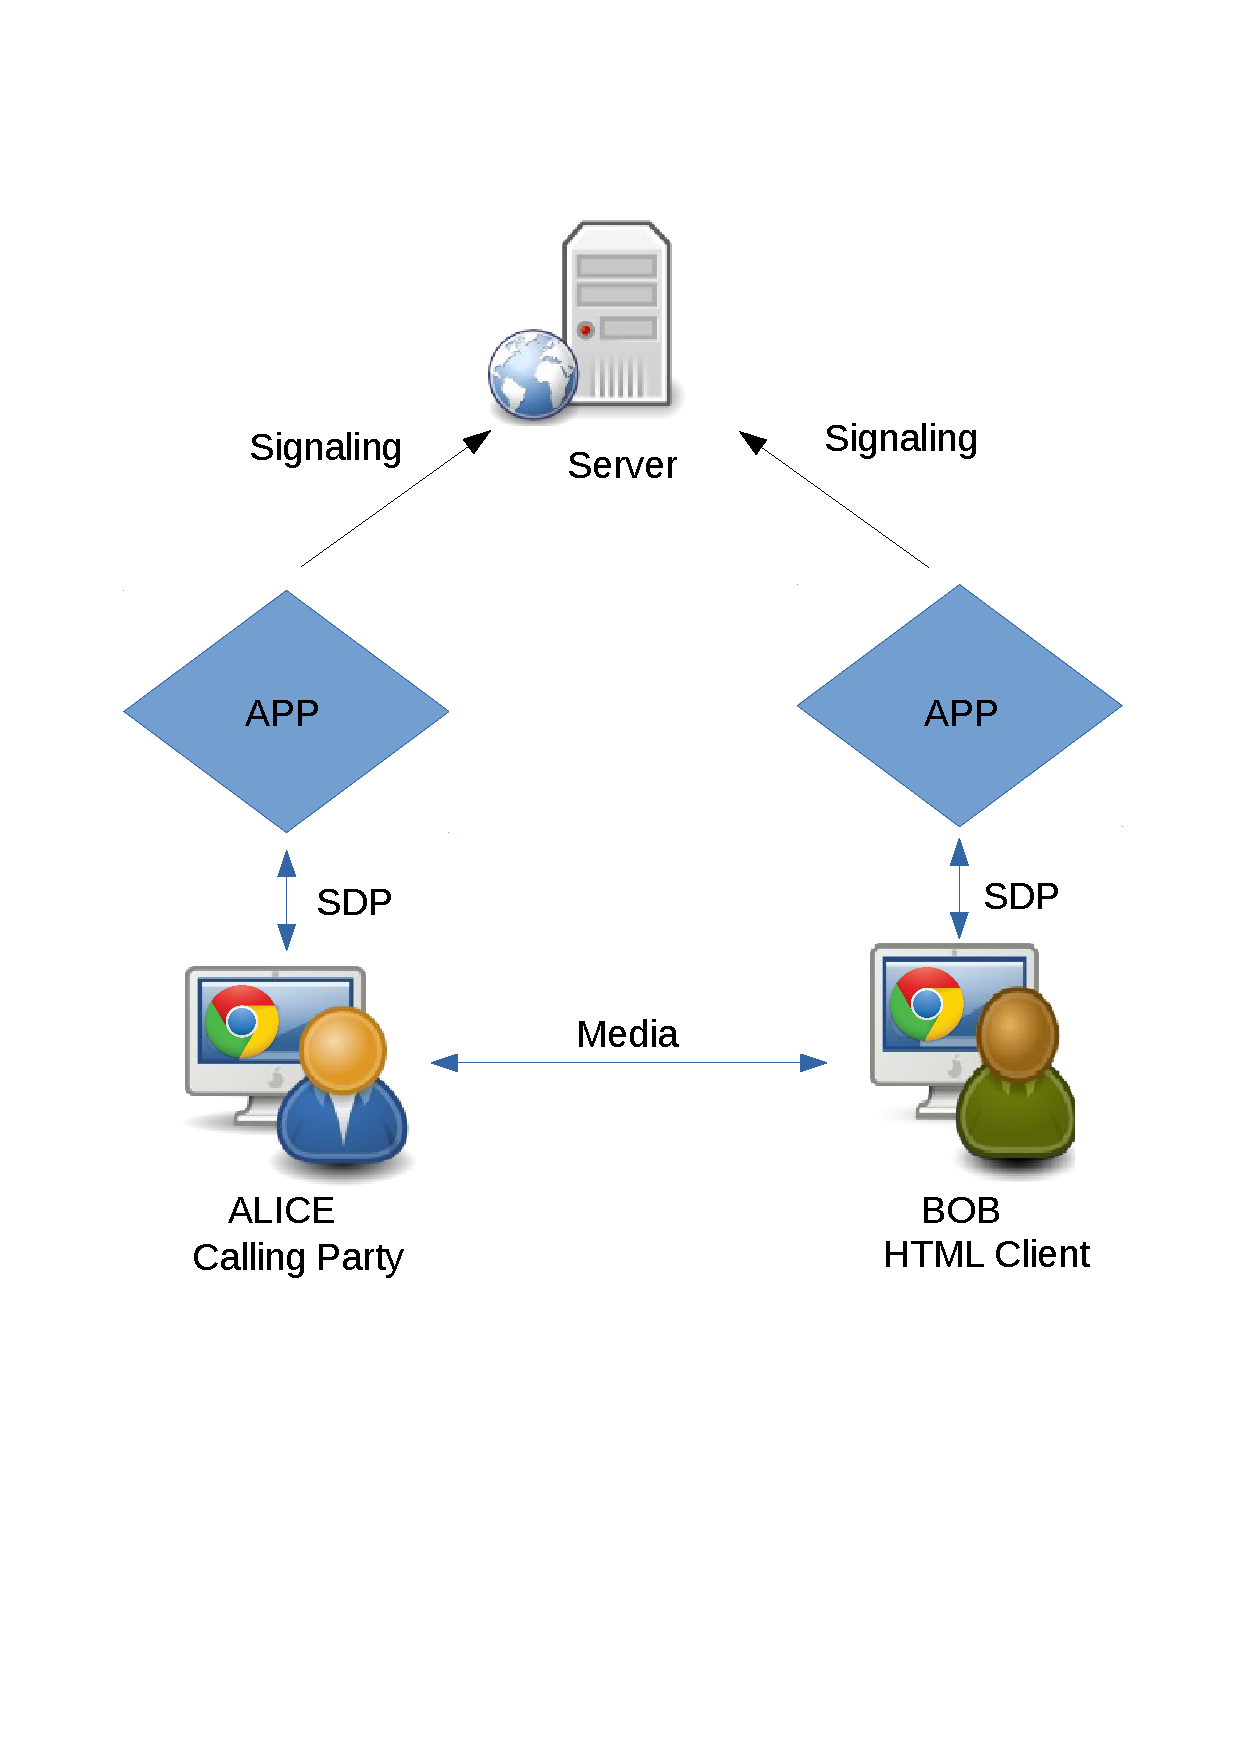
\includegraphics[width=1\columnwidth]{\webrtcdir/figures/figuras_ok/JSEP.pdf}
\end{column}
\end {columns}


\begin{itemize}

\item The offer/Answer contains the Session Description Protocol (SDP) that features all the characteristics to the data (video \& audio) to be exchanged:
  \begin{enumerate}
  \item Media (Audio \& Video) Codecs.
  \item Resolution format.
  \item Transport protocol used.
  \item Endpoint IP address and port.
  \item Other info to describe a media transfer endpoint.
  \end{enumerate}
\end{itemize}
\end{frame}


\begin{frame}[fragile]\frametitle{SDP}
\begin{itemize}
\item SDP Components:
  \begin{enumerate}
  \item Session Description
  \item Time Description
  \item Media Description
  \end{enumerate}
\item An SDP session description consists of a number of lines of text of the form:
\texttt{<type>=<value>}.

\item  where:
  \begin{enumerate}
  \item Type  must be exactly one case-significant character 
  \item Value is structured text whose format depends on <type>.  
  In general, <value> is either a number of fields delimited by a single space character or a free format string.  
  \item No white spaces allowed on both sides of "=" sign.
  \item Optional items are marked with a "*".
  \end{enumerate}
\end{itemize}
\end{frame}

\begin{frame}[fragile]\frametitle{SDP Example}
\begin{itemize}
\item SDP example:

\begin{lstlisting}[style=verbt]
v=0;
o= jdoe 2890844526 2890842807 IN IP4 10.47.16.5;
s= SDP WebRTC Alex-Gerard;
i= A example of SDP used in WebRTC;
u=http://Alex-Gerard-EetWebRTC-PFG.com;
e=j.eetwebrtc@gmail.com (Alex Albas, Gerard Auguets);
c=IN IP4 224.2.17.12/127;
t=2873397496 2873404696;
m= audio 54609 UDP/TLS/RTP/SAVPF;
a=rtpmap:0 PCMU/8000;
a=rtcp-mux; \\Alice can perform RTP/RTCP Mux
a=rtcp:54609 IN IP4 24.23.204.141 \\Port for RTCP data
a=ptime:60   \\Audio packetization of 60 ms
a=sendrecv \\Alice can send and receive audio
a=setup:actpass \\Alice can perform DTLS before answer arrives
a=fingerprint:sha-1 99:41:49:83:4a:97:0e:1f:ef:6d:f7:c9:c7:70:
9d:1f:66:79:a8:07 \\DTLS Fingerprint for SRTP
a=ice-ufrag:074c6550 \\ICE user fragment 
a=ice-pwd:a28a397a4c3f31747d1ee3 \\ICE password       
a=candidate:0 1 UDP  2122194687 
192.168.1.4 54609 typ host \\RTP Host Candidate
a=candidate:0 2 UDP 2122194687        
192.168.1.4 54609 typ host \\RTCP Host Candidate    
a=candidate:1 1 UDP  1685987071 24.23.204.141 64678 typ srflx        
addr 192.168.1.4 rport 54609  \\RTP Server Reflexive ICE Candidate 
a=candidate:1 2 UDP  1685987071 24.23.204.141 64678 typ srflx 
raddr 192.168.1.4 rport 54609\\RTCP Server Reflexive Candidate
a=rtcp-fb:109 nack \\Indicates NACK RTCP feedback support
a=rtcp-rsize Alice intends to use reduced size RTCP for this session   
\end{lstlisting}
  

\end{itemize}
\end{frame}

% TODO: He intentado poner el SDP example pero queda muuuy grande y feo.


\begin{frame}[fragile]\frametitle{Example}
\begin{itemize}
%TODO: Aqui tendriamos que poner que setRemote/LocalDescription y la offer viene generada por RTCPeerConnection que se explicará en las APIS de WebRTC, pero 
% que entra en el proceso de signaling.
\item The initial signaling steps:
  \begin{enumerate}
  \item Alice wants to reach Bob's browser, so an Offer is created and sent to the Server.
  \item Alice adds its offer to setLocalDescription(). %Importante comentar que se explicara mas abajo el setLocalDescription() y SDP.
  \item Bob reach the server and receive the offer generated by Alice.
  \item Bob adds to its setRemoteDescription() the received offer and create an answer to the server.
  \item Bob adds its answer to its setLocalDescription().
  \item Alice receive the answer from Bob and adds it to its setRemoteDescription().
   \end{enumerate}
%Comentar que este proceso (el de arriba) se hace al iniciar una llamada o si se esta reconfigurando la misma.
\end{itemize}
\end{frame}

\begin{frame}[fragile]\frametitle{Initial Scenario}
\begin{figure}
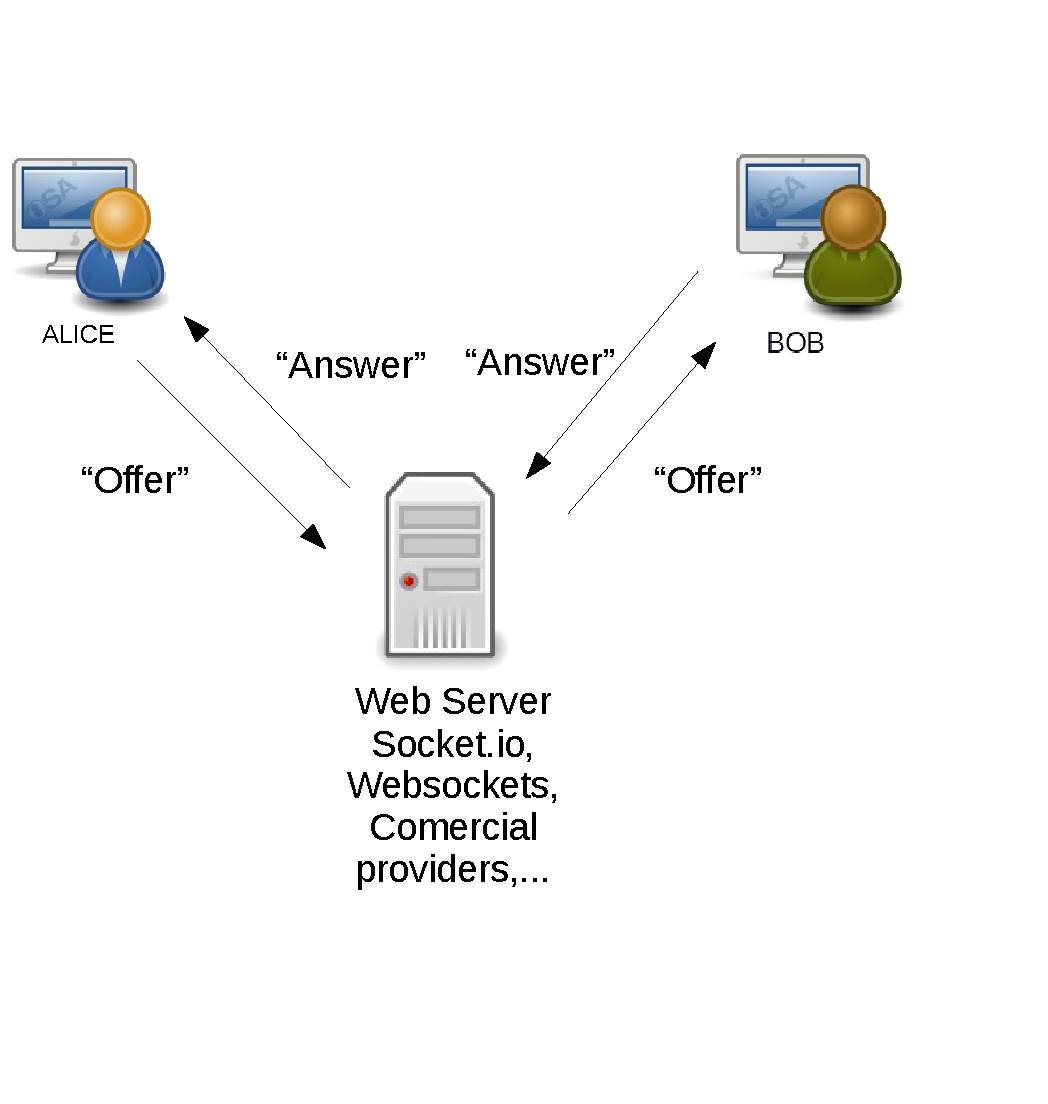
\includegraphics[width=0.7\textwidth]{\webrtcdir/figures/figuras_ok/4_signalling_offer_answer.pdf}
\end{figure}
%TODO: Igual se tendria que modificar la figura añadiendo el setLocalDescription ya que dentro de la offer/answer va el sdp.
\end{frame}


\begin{frame}[fragile]\frametitle{ICE Candidates}
\begin{itemize}
\item Peers must exchange information about the network connection. This is
known as an \textbf{ICE Candidate} and it details the available methods that the peer is
able to communicate (directly or through a TURN server). 
\item In other words, look for the best way to reach the other part through:

%* Interactive Connectivity Establishment.
%Tocaria explicar que es un STUN y un TURN
  \begin{enumerate}
  \item Stun Server.
  \item Turn Server.
  \end{enumerate}

\item The claim of ICE candidates is discover which transport address are valid, so \textbf{ICE framework} will try to find the best ICE candidate until works.
\item Once Offer/Answer have been sent:
  \begin{enumerate}
  \item ICE Candidate is going back and forward between Alice and Bob by the
  Signaling Server.
  \item Generally both could get an public IP, but if there is a firewall in the middle,
  other IP is given.
  \item When an ICE candidate is ready, it is possible to establish an \textbf{RTCPeerConnection}.
  \end{enumerate}
  
\end{itemize}
\end{frame}

\begin{frame}[fragile]\frametitle{Initial Scenario}
\begin{figure}
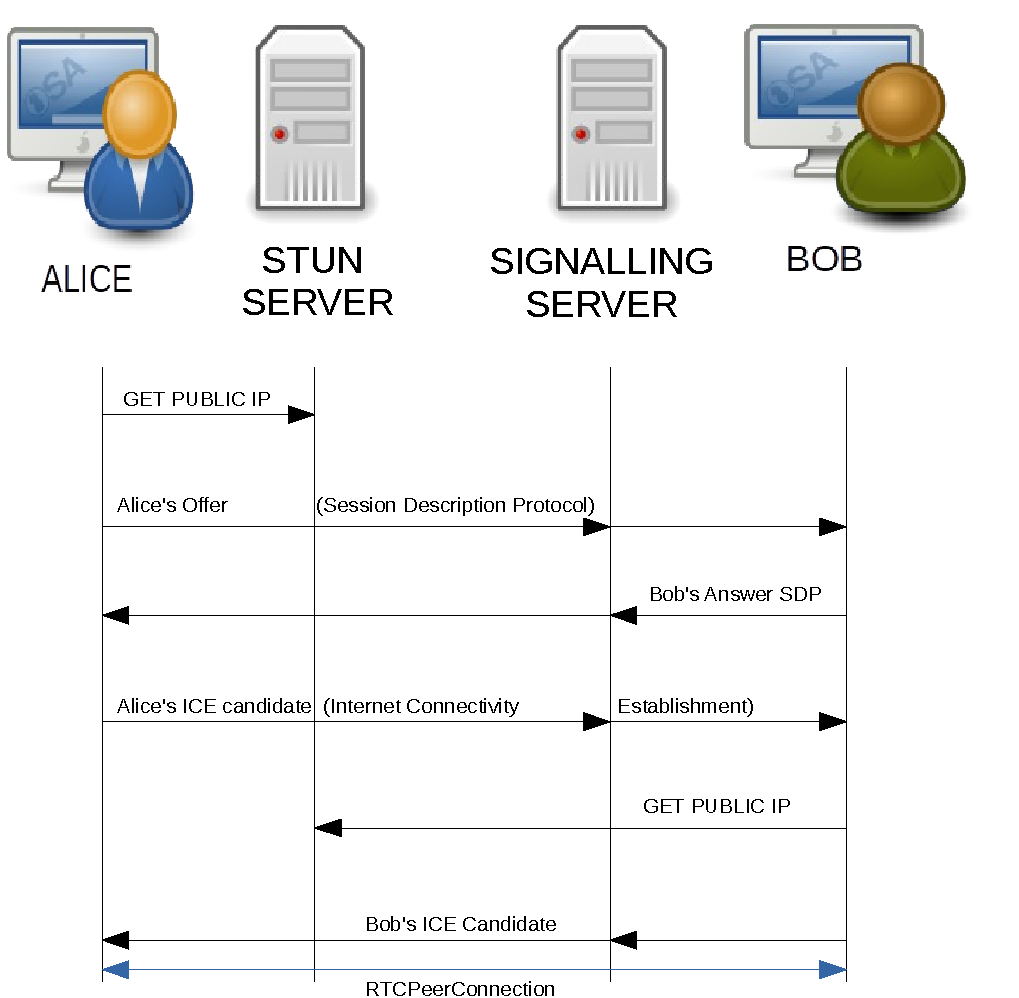
\includegraphics[width=0.6\textwidth]{\webrtcdir/figures/figuras_ok/4_signalling_diagram.pdf}
\end{figure}
\end{frame}

%% A PARTIR GERARD 

\section{WebRTC API's}

%FIXME By Jose: esta frame sin acabar????
% \begin{frame}[fragile]\frametitle{Introduction}
% WebRTC consist of several interrelated API's and protocols which work together to support 
% the exchange of data and media between two or more clients.

\begin{frame}[fragile]\frametitle{WebRTC API's}
\begin{itemize}
%FIXME By Jose: Error faltaba el \item aqui!!!!!!
\item There are three main categories of API that exist in WebRTC.
  \begin{itemize}
  \item Acquiring audio and video
  \item Communicating audio and video
  \item Communicating arbitrary data
  \end{itemize}
\item Because this three categories, WebRTC has three primary objects in order to acces to this components.
  \begin{itemize}
  \item MediaStream API
  \item RTCPeerConnection API
  \item RTCDataChannel API
  \end{itemize}
\end{itemize}
\end{frame}

\subsection{MediaStream API}
\begin{frame}[fragile]\frametitle{getUserMedia Method}
\begin{itemize}
\item This API is the responsible for managing all the media sources of the laptop, for example
the video of the webcam and the audio of the microphone.
\item Thanks to the MediaStream API the user can get access to all the laptop devices using the 
getUserMedia() method.
\end{itemize}
\end{frame}

\begin{frame}[fragile]\frametitle{Example}
\begin{itemize}
\item The following code shows a simple getUserMedia implementation:
\end{itemize}
\begin{lstlisting}[style=JavaScript]
var constraints = {video: true};

function succesCallback(stream) {
var video = document.querySelector("video");
video.src = window.URL.createObjectURL(stream);
}

function errorCallback(error){
console.log("navigator.getUserMedia error ", error);
}

navigator.getUserMedia(constraints,succesCallback, errorCallback);
\end{lstlisting}
\end{frame}

\begin{frame}[fragile]\frametitle{Mediastream}
\begin{itemize}
\item A MediaStreamTrack is a single source media element with an unique ID for example
the audio stream provided by the microphone.
\item A MediaStream Represents a single source of synchronized audio, video or both.
Each MediaStream contains one or more MediaStream tracks. 
\end{itemize}

\begin{figure}[htb]
\begin{centering}
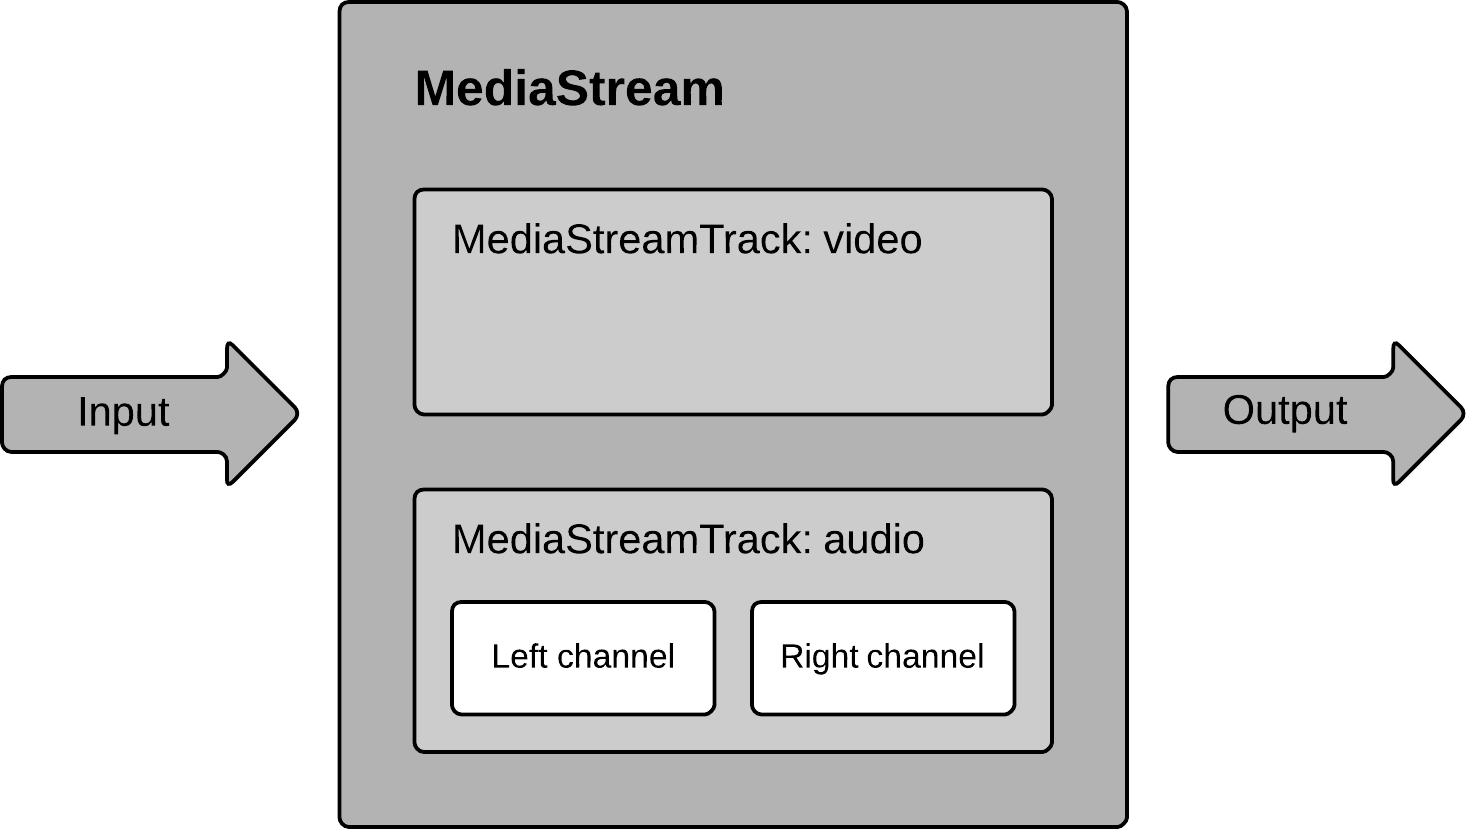
\includegraphics[width=0.7\columnwidth]{\webrtcdir/figures/figuras_ok/mediaStream.png}
\par\end{centering}
\end{figure}
\end{frame}


\subsection{RTCPeerConnection API}

\begin{frame}[fragile]\frametitle{Introduction}
\begin{itemize}
\item RTCPeerConnection:
\item The interface represents a WebRTC connection between peers, 
maintain and monitor the connection, and close the connection once it's no longer
needed.
\item This API doesn't handle the signaling process %this means that the user is completely 
%free to choose any signaling method.
\item The main functionality of this application is to transmit the acquired flow by
the getUserMedia API and send it to the other peer.
\item Management of all the parameters necessary to carry out transmission of multimedia data 
stream.
\end{itemize}
\end{frame}

\begin{frame}[fragile]\frametitle{RTCPeerConnection handling}
It is responsible for managing the following:	
\begin{itemize}
\item Signal processing and voice engine to remove noise from audio and video data 
and provide echo cancellation.
\item Codec handling and video engine.
\item Compression and decompression of audio and video.
\item Transport and Peer to peer communication in order to find the optimal route through firewalls, 
NATs and relays.
\item Security, encrypting the data to guarantee secure communications.
\item Bandwidth management. 
\end{itemize}
\end{frame}


\begin{frame}[fragile]\frametitle{RTCPeerConnection flow}
\begin{enumerate}
\item RTCPeerConnection API only has to send and receive MediaStreamTracks over a peer-to-peer connection.
\item The encoding of MediaStreamTracks is managed by objects called RTCRtpSenders.
\item The reception and decoding of MediaStreamTracks is managed through objects called RTCRtpReceivers.
\item When a MediaStreamTrack is attached to a RTCPeerConnection, 
a RTCRtpSenders object is created to be associated with this MediaStreamTrack.
\item RTCRtpReceivers  are created when remote signaling indicates 
that there are new tracks available.
\item The MediaStreamTrack and its associated RTCRtpReceivers are surfaced 
to the application.
\end{enumerate}
\end{frame}

\subsection{RTCDataChannel}

\begin{frame}[fragile]\frametitle{Introduction}
\begin{itemize}
\item Sending information is present in many areas like communications, file transfer and video games.
This requires fast communications, low-latency and guaranteeing the security of the data.
\item Currently there are other data channels as Websockets, Ajax and many more, but these technologies are designed for client/server
communications.
\item RTCDataChannel works directly with the RTCPeerConnection API.
\item RTCDataChannel is designed to replicate exactly the Websockets technology.
\end{itemize}
\end{frame}

\begin{frame}[fragile]\frametitle{Transmission Modes}
\begin{enumerate}
\item \textbf{Unreliable mode}: This mode does not guarantee the correct transmission of all the packets because works through UDP protocol, but 
eliminates the overhead so it is a faster mode, especially useful for gaming applications.

\item \textbf{Reliable mode}: This mode guarantee the transmission and order of all the packets because works through TCP protocol, but 
adds overhead in order to handling the control and error flow.
\end{enumerate}
\end{frame}


\begin{frame}[fragile]\frametitle{RTCDataChannel Example}
\begin{lstlisting}[style=JavaScript]
var peerConnection = new RTCPeerConnection();
var dataChannel =
  peerConnection.createDataChannel("STUN SERVERS", dataChannelOptions);

dataChannel.onerror = function (error) { //Manages error handling
  console.log("Data Channel Error:", error);
};
dataChannel.onmessage = function (event) { //Specifies a function to be called when the message event is fired on the channel.
  console.log("Got Data Channel Message:", event.data);
};
dataChannel.onopen = function () { //Manages the channel aperture
  dataChannel.send("Hello World!");
};
dataChannel.onclose = function () {
  console.log("The Data Channel is Closed"); //Manage the channel closure
};
\end{lstlisting}
\end{frame}


\section{Security}

\begin{frame}[fragile]\frametitle{Introduction}
\begin{itemize}
\small
\item WebRTC implementations can transfer sensitive content.
\item Ensuring communications security is a fundamental requirement for this type of applications.
\item The WebRTC architecture assumes from a security perspective that network resources exist in a 
hierarchy of trust.
\item The browser's job is to enable access to the Internet providing adequate security protections to the user. 
\item The browser is the portal through which the user accesses all WebRTC applications and content.
\item The level of trust provided to the user by WebRTC is directly influenced by the user's trust in the browser.
\end{itemize}
\end{frame}

\begin{frame}[fragile]\frametitle{WebRTC Security Mechanisms}
\begin{itemize}
\item WebRTC is not a plugin.
\item The browser can access local resources. WebRTC combat this by requiring the user to give explicit permission to the user.
\item When either the microphone or camera is being used the client UI is required to expressly show the user that the microphone 
or camera are being operated.
\end{itemize}
\end{frame}

\begin{frame}[fragile]\frametitle{HTTPS}
\begin{itemize}
\item HTTPS (Hypertext transfer protocol secure) is a communication protocol that uses the HTTP (Hypertext transfer protocol secure) and the SSL/TLS
(Secure sockets layer/Transport layer security) protocols to provide encrypted communication and secure identification of a Web Server.
\item This technology consist of communication over HTTP within a connection encrypted by transport layer security or secure sockets layer.
\item It creates a secure channel over an insecure network.
\item HTTP operates at the application layer. 
\end{itemize}
\end{frame}

\begin{frame}[fragile]\frametitle{HTTPS encryption \& DTLS}
\begin{itemize}
\small
\item Full encryption P2P.
\item The encryption protocol used depends on the channel type.
  \begin{enumerate}
  \footnotesize
  \item Data streams are encrypted using Datagram Transport Layer Security (DTLS).
  \item Media streams are encrypted using Secure Real-time Transport Protocol (SRTP).
  \end{enumerate}
\item DTLS is a standardized protocol used in email and voip communications to encrypt information. 
\item Offers full encryption with asymmetric cryptography methods,data authentication and message authentication.
\item SRTP is used for the mediaStreams encryption because is a lighter-weight option than DTLS.
\item SRTP uses AES,as a symmetric-key algorithm, meaning the same key 
is used for both encrypting and decrypting.
\end{itemize}
\end{frame}

\section{Implementation}
\subsection{Setting Up Server}

\begin{frame}[fragile]\frametitle{Server Side}
\begin{itemize}
 \item In the following code all the modules needed are imported using the require() method.
  \begin{lstlisting}[style=JavaScript]
  //Getting the modules
  var https = require('https');
  var fs = require('fs');
  var path = require('path');
  var express = require('express.io');
  \end{lstlisting}
\end{itemize}
\end{frame}

\begin{frame}[fragile]\frametitle{Server Side}
\begin{itemize}

 \item In order to enable the server to handle HTTPS connections, the server need to read the keys and certificates
created through OPENSSL based on Linux.
  \begin{lstlisting}[style=JavaScript]
  $ openssl genrsa 1024 > file.pem //Generating RSA KEY.
  $ openssl req -new -key file.pem -out csr.pem 
  //Input data in order to generate crs.pem
  $ openssl x509 -req -days 365 -in csr.pem -signkey file.pem -out file.crt 
  //SSL certificate saved
  \end{lstlisting}


\item Uses of .pem \& .crt using relative paths.

  \begin{lstlisting}[style=JavaScript]
  //Key & Certificate for https server.
  var options = {
	key:fs.readFileSync('./cert/file.pem'),
	cert:fs.readFileSync('./cert/file.crt')
  };
  \end{lstlisting}
\end{itemize}
\end{frame}

\begin{frame}[fragile]\frametitle{Server Side}
\begin{itemize}

\item HTTPS server creation, request and response.
\begin{lstlisting}[style=JavaScript]
//Server Creation
app.https(options).io();

//Defined HTTPS server port
var PORT = 8102; 
console.log('server started and listen to port: ' + PORT);

//Ask for static files on the public directory
app.use(express.static(path.join(__dirname, 'public')));

//When a request comes index.ejs is provide to the client
app.get('/', function(req, res){ 
    res.render('index.ejs');
});
\end{lstlisting}
\end{itemize}
\end{frame}

\begin{frame}[fragile]\frametitle{Server Side}
\begin{itemize}
 \item Every time that a client connect/disconnect to the server a message on the console of the server
will be printed.
\begin{lstlisting}[style=JavaScript]
//Display on the console connected/disconnected users
app.io.on('connection' , function(socket){
    console.log("A user connected!!");
    socket.on('disconnect', function() {
    // make your disconnection actions
    console.log("User disconnected!!");
    })
})
\end{lstlisting}
\end{itemize}
\end{frame}

\begin{frame}[fragile]\frametitle{Server Side}
\begin{itemize}

\item Joining into the room introduced by the user at the beginning of the connection.

\begin{lstlisting}[style=JavaScript]
//message other clients when some new user enter to the chatroom
app.io.route('ready', function(req){
    //req.data bring the name of the room (for textchat and signaling room)
    req.io.join(req.data.chat_room);
    req.io.join(req.data.signal_room);
    req.io.join(req.data.files_room);
    //Send a broadcast message to the room with name req.data
    app.io.room(req.data).broadcast('announce', {
        message:'New client in the ' + req.data + 'room.'
    });    
})
\end{lstlisting}
\end{itemize}
\end{frame}
\begin{frame}[fragile]\frametitle{Server Side}
\begin{itemize}
 \item This function set up the listening port able to receive connections:
\begin{lstlisting}[style=JavaScript]
app.listen(PORT);
\end{lstlisting}

\item Similar to text-chat Implementation.
Key difference:The sender will not receive his own message because of using req() method instead off app.io.room.
\begin{lstlisting}[style=JavaScript]
//Signaling process
app.io.route('signal', function(req){
    req.io.room(req.data.room).broadcast('signaling_message', {
        type:req.data.type, 
        message:req.data.message});
})
\end{lstlisting}
\begin{lstlisting}[style=JavaScript]
 
\end{lstlisting}
\end{itemize}
\end{frame}

\begin{frame}[fragile]\frametitle{Server Side}
\begin{itemize}

\item For the text chat Broadcast message to all the clients (sender included), that are connected in to the same room.
\begin{lstlisting}[style=JavaScript]
//Sending text messages to the connected clients 
app.io.route('send', function(req){
    app.io.room(req.data.room).broadcast('message', {
        message:req.data.message,
        author:req.data.author});
        })
\end{lstlisting}
\end{itemize}
\end{frame}


\subsection{Setting Up Client}

\begin{frame}[fragile,allowframebreaks]\frametitle{Client Side}
 Main Aspects:
\begin{itemize}
 \item The Core: Creating The RTCPeerConnection on the signaling process: %Aquí hay que explaiarse.
 
 \begin{lstlisting}[style = JavaScript]
//Setting up the RTC Peer Connection object
if (!rtcPeerConn) {
console.log("Start Signaling?");
startSignaling();
console.log('Yes, Signalingng has been started!!');
}
if (data.type != "user_here") {
var message = JSON.parse(data.message);
  if (message.sdp) {
    rtcPeerConn.setRemoteDescription(new RTCSessionDescription(
  message.sdp), function () {
  //if we have received an offer, we need to answer
  if (rtcPeerConn.remoteDescription.type == 'offer') {
  rtcPeerConn.createAnswer(sendLocalDesc, logError);
  }
  }, logError);
  } else {
    rtcPeerConn.addIceCandidate(new RTCIceCandidate(message.candidate));
  }
  }
});
 
 \end{lstlisting}

\end{itemize}
\end{frame}

\begin{frame}[fragile,allowframebreaks]\frametitle{StartSignaling Method}
\begin{itemize}
 \item Starting the signaling process: 
 
 \begin{lstlisting}[style = JavaScript]
function startSignaling() {
displaySignalMessage("starting signaling...");
rtcPeerConn = new RTCPeerConnection(configuration,null);
//Send any ice candidates to the other peer
rtcPeerConn.onicecandidate = function (evt) {
if (evt.candidate) {
io.emit('signal', {
"type": "ice candidate",
"message": JSON.stringify({
'candidate': evt.candidate
}),
"room": SIGNAL_ROOM
});
displaySignalMessage("Completed that ICE
candidate");
}
};
//let the 'negotiationneeded' event trigger offer
generation (SDP offer)
rtcPeerConn.onnegotiationneeded = function () {
displaySignalMessage("on negotiation called");
rtcPeerConn.createOffer(sendLocalDesc, logError);
};

//Once remote stream arrives, show it in the remote
video element
rtcPeerConn.onaddstream = function (evt) {
displaySignalMessage("going to add their stream...
");
theirVideoArea.src = URL.createObjectURL(
evt.stream);
};
  
 \end{lstlisting}

\end{itemize}
\end{frame}

\begin{frame}[fragile]\frametitle{GetUSerMedia}
\begin{itemize}
 \item Getting the media when the Signaling process has been completed.
 
 \begin{lstlisting}[style = JavaScript]
//This goes inside startSignaling() function.
navigator.getUserMedia({
'audio': true,
'video': true
//Once the stream is created, display in myVideo
tag, and add our stream as a source of audio/
video to our RTCPeerConn
}, function (stream) {
displaySignalMessage("going to display my
stream...");
//Adding the local stream to the video tag.
myVideoArea.src = URL.createObjectURL(stream);
//
rtcPeerConn.addStream(stream);
}, logError);

  
 \end{lstlisting}

\end{itemize}
\end{frame}

\section{Testing}

\begin{frame}[fragile]\frametitle{Testing}
\begin{itemize}
\item LET'S TRY
\end{itemize}
\end{frame}


\section{Conclusions}
\begin{frame}[fragile]\frametitle{Testing}
\begin{itemize}
\item Satisfactory results for the project development and the system implementation.
\item Academic-oriented.
\item Successfully technical knowledge.
\item WebRTC fulfill generated expectations.
\end{itemize}
\end{frame}


%FIXME By Jose comento a partir de aqui....
% 
% % 
% % 
% % 
% % 
% % \section{Security}
% % 
% % \begin{itemize}[htb]
% %  \item Acquiring audio and video
% %  \item Communicating audio and video
% %  \item Communicating arbitrary data
% % \end{itemize}
% \item Peers must exchange information about the network connection. This is
% known as an \textbf{ICE Candidate*} and it details the available methods that the peer is
% able to communicate (directly or through a TURN server). 
% \item In other words, look for the best way to reach the other part through:
% 
% %* Interactive Connectivity Establishment.
% %Tocaria explicar que es un STUN y un TURN
%   \begin{enumerate}
%   \item Stun Server.
%   \item Turn Server.
%   \end{enumerate}
% 
% \item The claim of ICE candidates is discover which transport address are valid, so \textbf{ICE framework} will try to find the best ICE candidate until works.
% \item Once Offer/Answer have been sent:
%   \begin{enumerate}
%   \item ICE Candidate is going back and forward between Alice and Bob by the
%   Signaling Server.
%   \item Generally both could get an public IP, but if there is a firewall in the middle,
%   other IP is given.
%   \item When an ICE candidate is ready, it is possible to establish an \textbf{RTCPeerConnection}.
%   \end{enumerate}
%   
% \end{itemize}
% \end{frame}
% 
% \begin{frame}[fragile]\frametitle{Initial Scenario}
% 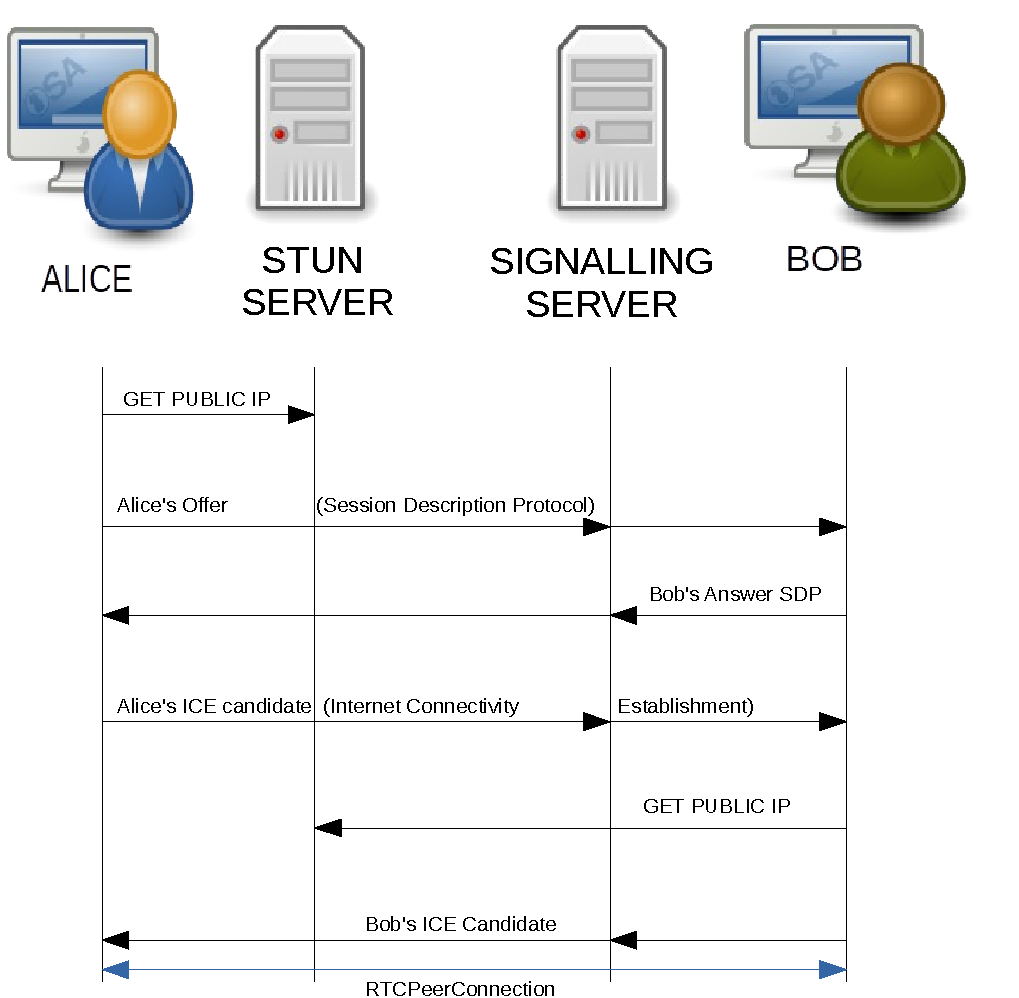
\includegraphics[width=0.6\textwidth]{\webrtcdir/figures/figuras_ok/4_signalling_diagram.pdf}
% \end{frame}
% 
% \subsection{WebRTC API's}
% 
% \begin{frame}[fragile]\frametitle{to be defined}
% \begin{itemize}
% \item to be defined
% \end{itemize}
% \end{frame}
% 
% 
% \section{Security}
% \begin{frame}[fragile]\frametitle{to be defined}
% \begin{itemize}
% \item to be defined
% \end{itemize}
% \end{frame}
% 
% \section{Implementation}
% \subsection{Setting Up Server}
% \begin{frame}[fragile]\frametitle{Server Side}
% \begin{itemize}
% 
% 
%  \item In the following code all the modules needed are imported using the require() method.
%   \begin{lstlisting}[style=JavaScript]
%   //Getting the modules
%   var https = require('https');
%   var fs = require('fs');
%   var path = require('path');
%   var express = require('express.io');
%   \end{lstlisting}
% \end{itemize}
% \end{frame}
% 
% \begin{frame}[fragile]\frametitle{Server Side}
% \begin{itemize}
% 
%  \item In order to enable the server to handle HTTPS connections, the server need to read the keys and certificates
% created through OPENSSL based on Linux.
%   \begin{lstlisting}
%   $ openssl genrsa 1024 > file.pem //Generating RSA KEY.
%   $ openssl req -new -key file.pem -out csr.pem 
%   //Input data in order to generate crs.pem
%   $ openssl x509 -req -days 365 -in csr.pem -signkey file.pem -out file.crt 
%   //SSL certificate saved
%   \end{lstlisting}
% 
% 
% \item Uses of .pem \& .crt using relative paths.
% 
%   \begin{lstlisting}[style=JavaScript]
%   //Key & Certificate for https server.
%   var options = {
% 	key:fs.readFileSync('./cert/file.pem'),
% 	cert:fs.readFileSync('./cert/file.crt')
%   };
%   \end{lstlisting}
% \end{itemize}
% \end{frame}
% 
% \begin{frame}[fragile]\frametitle{Server Side}
% \begin{itemize}
% 
% \item HTTPS server creation, request and response.
% \begin{lstlisting}[style=JavaScript]
% //Server Creation
% app.https(options).io();
% 
% //Defined HTTPS server port
% var PORT = 8102; 
% console.log('server started and listen to port: ' + PORT);
% 
% //Ask for static files on the public directory
% app.use(express.static(path.join(__dirname, 'public')));
% 
% //When a request comes index.ejs is provide to the client
% app.get('/', function(req, res){ 
%     res.render('index.ejs');
% });
% \end{lstlisting}
% \end{itemize}
% \end{frame}
% 
% \begin{frame}[fragile]\frametitle{Server Side}
% \begin{itemize}
%  \item Every time that a client connect/disconnect to the server a message on the console of the server
% will be printed.
% \begin{lstlisting}[style=JavaScript]
% //Display on the console connected/disconnected users
% app.io.on('connection' , function(socket){
%     console.log("A user connected!!");
%     socket.on('disconnect', function() {
%     // make your disconnection actions
%     console.log("User disconnected!!");
%     })
% })
% \end{lstlisting}
% \end{itemize}
% \end{frame}
% 
% \begin{frame}[fragile]\frametitle{Server Side}
% \begin{itemize}
% 
% \item Joining into the room introduced by the user at the beginning of the connection.
% 
% \begin{lstlisting}[style=JavaScript]
% //message other clients when some new user enter to the chatroom
% app.io.route('ready', function(req){
%     //req.data bring the name of the room (for textchat and signaling room)
%     req.io.join(req.data.chat_room);
%     req.io.join(req.data.signal_room);
%     req.io.join(req.data.files_room);
%     //Send a broadcast message to the room with name req.data
%     app.io.room(req.data).broadcast('announce', {
%         message:'New client in the ' + req.data + 'room.'
%     });    
% })
% \end{lstlisting}
% \end{itemize}
% \end{frame}
% \begin{frame}[fragile]\frametitle{Server Side}
% \begin{itemize}
%  \item This function set up the listening port able to receive connections:
% \begin{lstlisting}[style=JavaScript]
% app.listen(PORT);
% \end{lstlisting}
% 
% \item Similar to text-chat Implementation.
% Key difference:The sender will not receive his own message because of using req() method instead off app.io.room.
% \begin{lstlisting}[style=JavaScript]
% //Signaling process
% app.io.route('signal', function(req){
%     req.io.room(req.data.room).broadcast('signaling_message', {
%         type:req.data.type, 
%         message:req.data.message});
% })
% \end{lstlisting}
% \begin{lstlisting}[style=JavaScript]
%  
% \end{lstlisting}
% \end{itemize}
% \end{frame}
% 
% \begin{frame}[fragile]\frametitle{Server Side}
% \begin{itemize}
% 
% \item For the text chat Broadcast message to all the clients (sender included), that are connected in to the same room.
% \begin{lstlisting}[style=JavaScript]
% //Sending text messages to the connected clients 
% app.io.route('send', function(req){
%     app.io.room(req.data.room).broadcast('message', {
%         message:req.data.message,
%         author:req.data.author});
%         })
% \end{lstlisting}
% \end{itemize}
% \end{frame}
% 
% \subsection{Setting Up Client}
% 
% \section{Testing}
% 
% \begin{frame}[fragile]\frametitle{to be defined}
% \begin{itemize}
% \item to be defined
% \end{itemize}
% \end{frame}
% 
% \section{Conclusions}
% 
% \begin{frame}[fragile]\frametitle{to be defined}
% \begin{itemize}
% \item to be defined
% \end{itemize}
% \end{frame}
